\section{Moorer's Business}
Un successivo studio sulla simulazione digitale dei riverberi è stato condotto da \emph{James A. Moore} intorno al 1979, pubblicando i suoi risultati  su Computer Music Journal ,Vol. 3, No. 2.
L’articolo, intitolato \emph{“About this Reverberation Business”}, tratta di ulteriori integrazioni e accorgimenti che possono essere applicati durante lo sviluppo di un riverbero.

L’autore, infatti, partendo dalla letteratura già presente, tra cui gli articoli di Schroeder e J.Chowning, sperimenta nuovi algoritmi, rendendo più snelli i precedenti, sempre tendendo ad una realisticità del riverbero.

Innanzitutto vengono ripresi i sistemi fondamentali dell’analisi di Schroeder, vale a dire, il filtro Comb (visto in figura \ref{fig:dfl}) e il filtro All Pass (visto in figura \ref{fig:apf}). Quest’ultimo in una seconda versione caratterizzata da una singola moltiplicazione, a fronte delle 3 precedenti, rendendolo più sostenibile a livello di computazione.

\begin{figure}[htp]
\centering
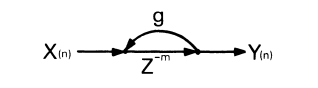
\includegraphics[width=%
0.60\textwidth]{combmoorer}
\caption{Filtro Comb di Moorer}
\label{fig:combmoorer}
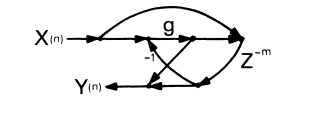
\includegraphics[width=%
0.60\textwidth]{apfmoorer}
\caption{Filtro All Pass di Moorer}
\label{fig:apfmoorer}
\end{figure}

Aventi le seguenti funzioni di trasferimento:
\begin{equation}
T(z) = \frac{g + z^{-m}}{1+gz^{-m}}
\end{equation}
\begin{equation}
T(z) = \frac{z^{-m}}{1-gz^{-m}}
\end{equation}

Osservando la funzione trasferimento dell’All Pass possiamo notare come il coefficiente del numeratore sia in ordine inverso di quello al denominatore, forzando gli zeri ad essere reciproci dei poli, definendo il comportamento All Pass del filtro.

Seguendo il lavoro fatto da Schroeder, per utilizzare i sistemi come riverberatori è necessario utilizzare una combinazione degli stessi.

Le combinazioni sono le medesime viste in precedenza e proposte da Schroeder (fig \ref{fig:apfseq} e \ref{fig:comballpass}). Parliamo dunque di una serie di All Pass nel primo algoritmo e, una cascata di comb filter seguiti da 2 All Pass nel secondo

\begin{figure}[htp]
\centering
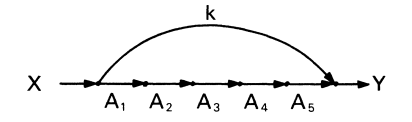
\includegraphics[width=%
0.60\textwidth]{allallpass}
\caption{Filtro Comb di Moorer}
\label{fig:allallpass}
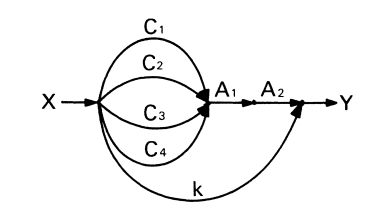
\includegraphics[width=%
0.60\textwidth]{comballpassmoorer}
\caption{Filtro All Pass di Moorer}
\label{fig:comballpassmoorerB}
\end{figure}

\subsection{Problematiche Del riverberatore}

Il riverberatore così ottenuto, però, non rispecchia alcune caratteristiche desiderate, portando ad aberrazioni acustiche non presenti in natura.
Le problematiche riscontrate possono essere riassunte in:

\begin{itemize}
\item riverberazione non ottimale per suoni impulsivi e con transienti molto corti, producendo pattern ritmici composti dagli echi al posto di un riverbero uniforme;
\item riverberazione con un carattere metallico, soprattutto per tempi molto lunghi;
\end{itemize}

A questo punto l’autore considera l’utilizzo di nuove unità riverberanti, ma comunque mantenendo la struttura Comb-All Pass, ritenuta la migliore in termini di risposta.

\subsection{Nuove unità riverberanti}

Nel corso delle sue sperimentazioni Moorer costruisce altre 4 unità riverberanti, alcune molto simili tra di loro in quanto i concetti alla base restano i medesimi. In particolare, l’intuizione dell’autore è stata quella di introdurre un ulteriore filtro all’interno dei feedback.

Lo scopo del filtro, ricollegandoci agli argomenti trattati nei capitoli precedenti, è quello di simulare l’attenuazione delle alte frequenze causate dall’aria. Come già detto, è un coefficiente che, in base a caratteristiche quali umidità e temperatura, sottrae energia alle alte frequenze dello spettro, scurendo quest’ultimo.

\subsection{Nuove unità riverberanti}

Come detto, le unità proposte sono 4, ma una in particolare sembra essere la più efficiente, ovverosia:

\begin{figure}[htp]
\centering
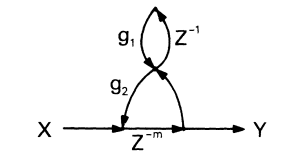
\includegraphics[width=%
0.50\textwidth]{combfiltro}
\caption{Filtro Comb con all'interno un filtro Passa Basso}
\label{fig:combfiltro}
\end{figure}

Come è possibile notare, si tratta di un Comb filter al cui interno è presente un filtro di tipologia Low pass $T(z)$. Il valore di $g_1$ controlla il roll-off del filtro e in seguito troveremo un modo per capire quale valore sarà più conveniente.
All’interno, i valori $g_1$ e $g_2$ seguiranno la condizione di $g_1+g_2<1$ per motivi di stabilità.

La risposta in frequenza, a detta di Moorer,  non sarà in grado di restituire un valore coerente alla realtà, in quanto il singolo filtro Low pass (di primo ordine) è un compromesso per rendere il tutto più efficiente.

Successivamente, nell’articolo viene anche consigliato di tenere in considerazione della modifica dei tempi di delay in base alle caratteristiche dell’aria (temperatura e umiditá), anche se nel testo si fa riferimento a valori standard e non modificabili.
I valori di $g$, dipendenti dall’umidità, sono in seguito esposti grazie agli studi di Moorer nel seguente grafico.
\begin{figure}[h!]
\centering
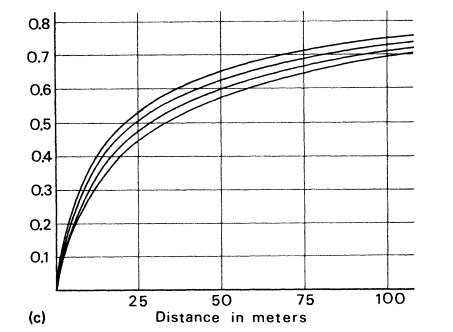
\includegraphics[width=%
0.50\textwidth]{assorbimentomoorer}
\caption{Grafico raffigurante l'andamento del valore di $g$ a causa dell'assorbimento dell'aria}
\label{fig:assorbimentomoorer}
\end{figure}
\bigskip
\subsection{In conclusione}
Moorer conclude la sezione riportando i risultati ottenuti. L’inserimento del filtro permette una miglior riverberazione per i suoni impulsivi, infatti il tempo di ogni eco risulta essere esteso, soprattutto per quanto riguarda le prime riflessioni e nascondendo i vuoti creati dalla bassa densità.
Il risultato sonoro non è particolarmente entusiasmante a detta dell’autore, ma sopperisce ad alcune mancanze delle precedenti iterazioni, rendendo questo sistema il più efficace al momento della scrittura.
